\documentclass{scrartcl}

\usepackage{amsmath, amsthm}
\usepackage{amsfonts}
\usepackage{amssymb}
\usepackage{arydshln}	%Array Dash Line
\usepackage{graphicx}
\usepackage{lipsum}
\usepackage[utf8]{inputenc}
\usepackage[ngerman]{babel}

\newtheorem{Def}{Definiton}
\newtheorem{Lem}{Lemma}
\newtheorem{Algo}{Algorithmus}

\newcommand{\BR}{\mathbb{R}}

\title{GAUSS}
\author{Felix Fl. und David B.}

\begin{document}

\maketitle

\tableofcontents
\newpage

\section{Der Gauss-Algorithmus}
Der Gauß-Algorithmus ist ein Algorithmus welcher eine gegebene Matrix $M$ in Zeilenstufenform bringt.

Eine derart umgeformte Matrix $M$ mag z.~B. so aussehen:
\[ M = \begin{pmatrix}
5 & 6 & 9 & 8\\ 
0 & 7 & 5 & 1\\ 
0 & 0 & 0 & 3
\end{pmatrix} \]

Aus der Zeilenstufenform einer Matrix lassen sich nun wesentliche Eigenschaften dieser Matrix ablesen.

Es ist demnach schnell ersichtlich dass der Gauß-Algorithmus ein essentielles Werkzeug beim Arbeiten mit Matrizen darstellt.
\subsection{Zeilenumformungen und Elementarmatrizen}

Für den Gauss-Algorithmus sind einige basische Zeilenumformungen innerhalb einer Matrix notwendig. Diese sind:

\begin{itemize}
\item Zeilenaddition
\item Zeilenmultiplikation
\item Zeilenvertauschung
\end{itemize}

Um diese verschiedenen Operationen auszuführen lässt sich die Matrix-Matrix-Multiplikation anwenden. Hierfür lassen sich drei verschiedene, im folgenden aufgeführte Matrizen $Q^i_j(\lambda)$, $S^i(\lambda)$ und $P^i_j$ definieren.
Um jedoch eben jene Matrizen zu definieren, muss zuerst die Matrix $E^i_j$ definiert werden als:


\textbf{TODODODO}
\subsubsection{Matrix $E^i_j$}
\begin{Def} Matrix $E^i_j$
\begin{align*}
 	E^i_j &=
	 	\begin{pmatrix}
	 	0 & \cdots & 0 \\
	 	\vdots & e_{ij} = 1 & \vdots \\
	 	0 & \cdots & 0 
 	\end{pmatrix}
\end{align*}
\end{Def}

% Raggedright um linksbündig zu bleiben
\vspace{8pt}

\raggedright Nun lassen sich die verschiedenen Zeilenumformungen folgendermaßen definieren:
\subsubsection{Zeilenaddition $Q^i_j(\lambda)$}
Bei der Zeilenaddition wird zur Zeile $i$ die Zeile $j$ mit Vorfaktor $\lambda$ hinzugefügt.
Die Matrix $Q^i_j(\lambda)$ ist folgendermaßen definiert:
\begin{Def} Zeilenaddition:
\begin{align*}
	Q^i_j(\lambda) & = & E_m + \lambda \cdot E^i_j \\
	Q^i_j(\lambda) & = & 
	\begin{pmatrix}
	1 & \cdots & 0 \\ 
	\vdots &  q_{ij} = \lambda & \vdots \\  
	0 & \cdots & 1
	\end{pmatrix} 
\end{align*}
\end{Def}
\raggedright
Um nun diese Elementarmatrix auf eine Matrix M anzuwenden, muss sie von links mit $M$ multipliziert werden: $Q^i_j(\lambda) \cdot M$
Das Ergebnis dieser Multiplikation ist nun eine neue Matrix, welche den Dimensionen der Matrix $M$ entspricht und dieselben Zeilen hat wie $M$, jedoch mit dem Unterschied dass zur Zeile $i$ die Zeile $j$ mit Vorfaktor $\lambda$ hinzugefügt wurde.

\subsubsection{Zeilenmultiplikation $S^i(\lambda)$}
Bei der Zeilenmultiplikation wird die Zeile $i$ in $M$ mit dem Faktor $\lambda$ multipliziert. Andere Zeilen werden hierbei nicht verändert. Die Matrix $S^i(\lambda)$ ist folgendermaßen definiert:
\begin{Def}
\begin{align*}
	S^i(\lambda) &=& E_m + (\lambda - 1) \cdot E^i_i \\
	S^i(\lambda) &=& 
	\begin{pmatrix}
	1 & \cdots & 0 \\ 
	\vdots & s_{ii} = \lambda & \vdots \\ 
	0 & \cdots & 1
	\end{pmatrix} 
\end{align*}
\end{Def}
\raggedright Um nun diese Elementarmatrix auf eine Matrix $M$ anzuwenden muss sie, wie bekannt, von links mit $M$ multipliziert werden: $S^i(\lambda) \cdot M$. 
Das Ergebnis dieser Multiplikation ist eine Matrix mit den Dimensionen von $M$, sowie den selben Zeilen, mit jedoch dem Unterschied dass die Zeile $i$ mit einem Vorfaktor $\lambda$ multipliziert wurde.

\subsubsection{Zeilenvertauschung $P^i_j$}
Bei der Zeilenvertauschung werden die Zeilen $i$ und $j$ miteinander vertauscht. Die daraus entstehende Matrix enthält noch beide Zeilen wie zuvor, jedoch an anderen Positionen. Die dazugehörige Matrix $P^i_j$ ist folgendermaßen definiert:
\begin{Def} Zeilenvertauschung:
\begin{align*}
	P_j^i(\lambda) &=& E_m - E^i_i - E^j_j + E^j_i + E^i_j \\
	P^i_j &=& 
	\begin{pmatrix}
	1 & \cdots & \cdots & 0 \\ 
	\vdots & E_{ii} = 0 & E_{ij} = 1 &  \\ 
	\vdots & E_{ji} = 1 & E_{jj} = 0 &  \\ 
	0 & \cdots & \cdots & 1
	\end{pmatrix} 
\end{align*}
\end{Def}
\raggedright Um nun Zeile $i$ und $j$ in einer Matrix $M$ zu vertauschen muss die Elementarmatrix $P^i_j$ von links an $M$ multipliziert werden: $P^i_j \cdot M$
Das Ergebnis dieser Multiplikation ist eine Matrix mit den Dimensionen von $M$ sowie den gleichen Zeilen, mit dem Unterschied dass die Zeilen $i$ und $j$ miteinander vertauscht wurden.

\subsection{Beispiel}
Dies ist ein Beispiel der Anwendung des Gaußalgorithmus.
Wir nehmen als  Ausgangsmatrix die $m\times n$ Matrix 
$A=\begin{vmatrix}
0 & 0 & 1 & 2 & 9 \\ 
0 & 3 & 4 & 5 & 9 \\ 
0 & 6 & 7 & 8 & 9 \\ 
0 & 9 & 9 & 9 & 9
\end{vmatrix} 
\leadsto

\subsection{Formulierung des Algorithmus}
\subsubsection{Der Gauß-Algorithmus allgemein formuliert}
\begin{Algo} Der Gauß-Algorithmus ist eine Reihe von Anweisungen welche nacheinander ausgeführt werden können um eine beliebige Matrix in Zeilenstufenform zu bringen.
	\begin{itemize}
		\item[Input:] $m \times n $ Matrix A , $a_j$ ist die $j$-te Spalte
		\item[Output:] $\tilde{A}$ in Zeilenstufenform (ZSF)
	\end{itemize}
\end{Algo}	
	\begin{enumerate}
		\item Zuerst wird geprüft ob die Matrix leer ist also ob $A=0$. Ist dies der Fall so ist Matrix  $A$ bereits in ZSF.
		\item Nun wird die Zählvariable $j$ auf $j=1$ gesetzt.
		\item Wenn die $j$-te Spalte leer ist also $a_j=0$ dann wird $j$ um eins erhöht $j+1\rightarrow j$ und dieser Schritt wiederholt.
		\item $k$ wird definiert als der erste Eintrag in der $a_j$-ten Spalte welcher ungleich Null ist $k:=min\{i|a_{ij}\neq0\}$.
		\item Ist nun $k\neq1$ so muss die $k$-te Zeile mit der ersten vertauscht werden um im nächsten Schritt fortzufahren zu können.
		\item Da $k\neq0$ ist es nun möglich mithilfe der Zeilenaddition und dem Faktor $\lambda=\frac{-a_{ij}}{\bar{a}_{1j}}$ alle Einträge unter $a_1j$ in Zeilen $2\leq{i}\leq{m}$
		zu eliminieren.
		\item Hiernach werden die Schritte 1 bis 6 mit der Untermatrix $A_2:=(a_{pq})_{\substack{2\leq p\leq m\\ j+1 \leq q \leq n}}$ wiederholt solange $m>1 \wedge n>1$
		\item $A$ ist in ZSF 
	\end{enumerate}
\subsubsection{Terminierung des Gauß-Algorithmus}
	Der Gauß-Algorithmus terminiert auf jeden Fall da mit jedem Durchlauf $m$ und $n$ abnehmen und streng monoton fallend sind und da die $m \times n$ Matrix $A$ endlich groß ist. 


\subsection{Anwendung: Invertierung einer Matrix}
Nebst seinen vielen Anwendungen zur Restrukturierung von Matrizen in eine Zeilen-Stufen-Form kann der Gauss-Algorithmus auch verwendet werden, um die Inverse einer quadratischen Matrix $M$ zu berechnen.
Dies ist folgendermaßen möglich:

\begin{itemize}
\item Man definiere zuerst eine neue Matrix $A$ folgendermaßen:
$A = (M|E_m)$
\item Diese neu definierte Matrix wird nun mithilfe des Gauss-Algorithmus so umgeformt, dass am Anfang der Matrix eine Einheitsmatrix $E_m$ steht.
\begin{itemize}
\item Ist dies nicht möglich, so kann die Matrix $M$ nicht invertiert werden.
\end{itemize}
\item Die daraus folgende Matrix $A_{Ergebnis}$ ist nun folgendermaßen aufgebaut: $A_{Ergebnis} = (E_m|M^{-1})$
\end{itemize}
Entfernt man nun die ersten $m$ Spalten der Matrix $A_{Ergebnis}$, so ist die verbleibende Matrix $A_{Schnitt}$ gleich der Inversen der Matrix $M$, d.h. $M^{-1}$

\begin{proof}
Um eine Matrix $M$ in die ZSF zu brigen, wendet der Gauss-Algorithmus eine Verkettung von Elementarmatrizen $(E_1 \cdots E_k)$ an.

Zudem liefert der Gauss-Algorithmus bei der Umformung von $(M|E_m)$ die Matrix $(E_m|B)$, d.h.: 
\begin{eqnarray*}
 (E_1 \cdots E_k) \cdot (M|E_m) &=& (E_m|B) \\
 \Leftrightarrow 
 ((E_1 \cdots E_k) \cdot A | (E_1 \cdots E_k)) &=& (E_m|B)
\end{eqnarray*}

Diese Formel lässt sich nun wie folgt aufspalten:
\begin{eqnarray*}
 B &=& (E_1 \cdots E_k) \\
(E_1 \cdots E_k) \cdot A &=& E_m
\end{eqnarray*}

Durch Ersetzung von $(E_1\cdots E_k)$ mit $B$, da diese Terme äquivalent sind (siehe oben), erhält man:
\[ B\cdot A = E_m \]

Da dies jedoch äquivalent ist zur Definition der Inverse einer Matrix, gilt:
\[ B=A^{-1}\]

\end{proof}


\section{Beispiele für die Anwendung der Linearen Optimierung}
Um uns in die Lineare Optimierung ein zu führen, wurden uns verschiedene Beispiele vorgestellt. Diese sollten wir als sog. Lineare Probleme, d.h. verschiedene Lineare Gleichungen und Ungleichungen definieren.
Diese Beispiele werden nun aufgeführt.

Im Folgenden betrachten wir das erste Beispiel, das Problem der Optimierung des Datenflusses innerhalb eines Netzwerkes.
\subsection{Netzwerk-Datenflussoptimierung}
	In dem gestellten Problem geht es darum ein Fluss von Daten von Eingang $o$ zu Ausgang $n$ über die Knoten $a$ bis $d$ größtmöglich zu gestalten unter Beachtung verschiedener Bedingungen.  Jeder Knoten hat nur Verbindungen zu bestimmten anderen Knoten bzw. Eingang und Ausgang wobei sie selbst nichts zwischenspeichern können. Diese Verbindungen können nur in eine Richtung benutzt werden und haben eine Höchstflussrate welche nicht überschritten werden darf.
	\includegraphics*[width=\textwidth]{Grafiken/Netzwerkflussbild.png}
	Also versuchen wir den Fluss zum letzten Knoten $o$ zu maximieren.Hierzu definieren wir $f_ij$ als der tatsächliche Fluss zwischen den Knoten $i$ und $j$.
	\[ \max(f_{do}+f_{eo}) \]
	Um die maximale Kapazität der Verbindungen zu beachten werden folgende Ungleichungen eingeführt.Hierbei sind $i$ und $j$ zwei Knoten zwischen denen eine Verbindung besteht. $k_{ij}$ beschreibt die maximale Kapazität und $f_{ij}$ den tatsächlichen Fluss. Daraus ergibt sich für alle möglichen zulässigen $i$ und $j$:  
	\begin{align*}
		-k_{ij} \leq f_{ij} \leq k_{ij}
	\end{align*}
	Dabei gelten die Nebenbedingungen das der Fluss von einem Knoten genauso groß sein muss wie der Fluss von dem Knoten weg. Die Flussrichtung wird mit Vorzeichen berücksichtigt. Hierbei ist $x$ ein beliebiger Knoten und $j$ alle Knoten mit denen er verbindet.
	\[
	0=\sum_{j=1}^{j_{max}{f_{xj}}
	\]
	Wird dieses Lineare Programm gelöst so erhält man einen maximalen Fluss. 
	
	
	
	
\subsection{Eisproduktionsplanung}
Das Problem der Eisproduktionsplanung befasst sich mit folgendem Szenario:

Man besitzt eine Eis-Firma, welche über den gesamten Verlauf des Jahres Eis produzieren soll. Da man jedoch keine Über- oder Unterproduktion, und damit Verluste, in Kauf nehmen möchte, versucht man mithilfe von Vorhersagen für das folgende Jahr seine Eisproduktion hieran anzupassen. Eine mögliche Vorhersage sieht folgendermaßen aus:

\centering
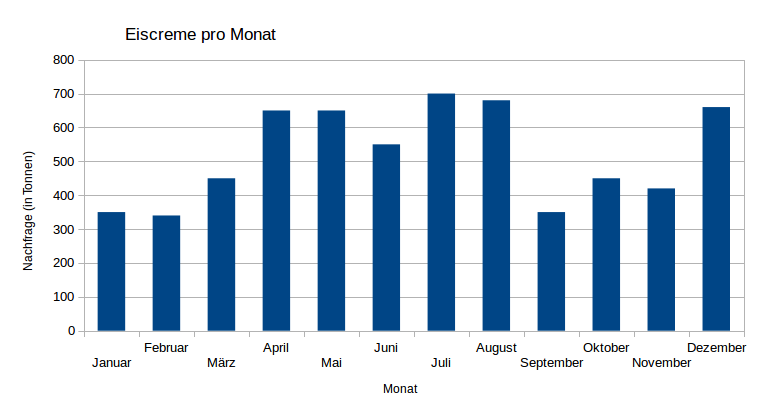
\includegraphics[width=\textwidth]{Grafiken/Eiscreme.png}

\raggedright
Bei der Erstellung der Linearen Ungleichung muss nun folgendes beachtet werden:

\begin{itemize}
\item Die Änderung der Produktionsmenge von Monat A zu Monat B kostet 50€ pro Tonne.
\item Eis lässt sich lagern, jedoch kostet dies 20€ pro Tonne pro Monat.
\item Die Produktion von einer Tonne Eis kostet 1€
\item Es darf keine Unterproduktion vorliegen, d.h. der Bedarf muss gedeckt werden.
\item Zu Anfang des Jahres gibt es kein Eis, und zu Ende des Jahres darf ebenso kein Eis mehr vorhanden sein.
\end{itemize}

Dies liefert folgende Bedingungen:
\begin{itemize}
\item Für einen Monat $m$ in $M$ muss die Produktionsmenge $p_m$, sowie die Menge der gelagerten Eiscreme $l_m$ größer als die Nachfrage $n_m$ sein:
\[ p_m + l_m \geq n_m \]
\item Die Menge des in einem Monat gelagerten Eises ist gleich der in vorherigen Monat übrig-gebliebenen Menge Eises:
\[ l_m = p_{m-1} + l_{m-1} - n_{m-1} \]
\item Die insgesamt produzierte Menge an Eiscreme muss gleich der gesamten Nachfrage sein:
\[ \sum p_m = \sum n_m \]
\item Die Änderung der Produktionsmenge $c_m$ ergibt sich aus der Differenz der Produktionsmenge des Monates und des vorherigen Monates: 
\[ c_m = p_{m} - p_{m-1} \] 
	\begin{itemize}
	\item Man muss hierbei beachten dass sowohl negative als auch positive Änderungen kosten! Da der Simplex-Algorithmus jedoch nur mit linearen Funktionen, d.h. ohne $\text{abs()}$ arbeiten kann, müssen zwei Hilfsvariablen, $cd_m$ und $ci_m$ (decrease und increase) aufgestellt werden:
	\begin{align*}
	c_m &= ci_m - cd_m \\
	ci_m &\geq 0		\\
	cd_m &\geq 0
	\end{align*}
	
	\item Die absolute Gesamtänderung der Produktionsrate kann nun mit $ci_m + cd_m$ errechnet werden.
 	\end{itemize}
\end{itemize}

Zudem will man die Gesamtkosten minimieren, d.h. :
\[ \min: \sum (1 \cdot p_m + 50 \cdot (ci_m + cd_m) + 20 \cdot l_m)\]

Will man dies nun mithilfe eines Solvers lösen wollen, so würde eine mögliche Implementation der Bedingungen folgendermaßen aussehen:
\newline

min $\sum\{m~in~M\} ~ (1 \cdot p[m] + 50 \cdot (ci[m] + cd[m]) + 20 \cdot l[m])$ \\
s.t. $\{m~in~M\} ~ p[m] + l[m] \geq n[m]$ \\
s.t. $\{m~in~M\} ~ l[m] = p[m - 1] + l[m - 1] - n[m - 1]$ \\
s.t. $\{m~in~M\} ~ \sum p[m] - n[m] = 0$ 	\\
s.t. $\{m~in~M\} ~ c[m] = p[m] - p[m-1]$ 	\\
s.t. $\{m~in~M\} ~ cd[m] \geq 0$			\\
s.t. $\{m~in~M\} ~ ci[m] \geq 0$			\\
s.t. $\{m~in~M\} ~ c[m] = ci[m] - cd[m]$	
\newline

solve;
\subsection{Berechnung einer optimalen Trennlinie}
In diesem Problem geht es darum mithilfe von Messwerten der Schattengröße und dem Gewicht eines Tieres zu bestimmen ob es ein Hase oder Wiesel ist.Man kann es graphisch vorstellen als würde man alle Messwerte in ein Diagramm eintragen und versuchen eine Gerade $y=mx+n$ zu finden die die Gruppen von Punkten trennt.
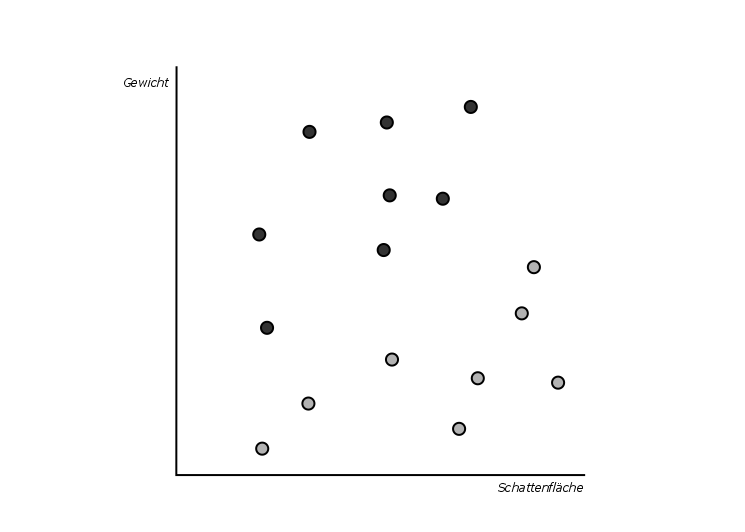
\includegraphics[width=\textwidth]{Grafiken/HaseWieselBild.png}
Dann würde gelten das \[y_h>mx_h+n\] für alle Hasen und \[
y_w<mx_w+n\] für alle Wiesel. Jedoch sind strikte Ungleichungen in linearen Programmen verboten. Deshalb wird eine Variable $\lambda$ eingeführt welche den Abstand zwischen allen Punkten und der Geraden beschreibt. Dies resultiert in den Ungleichungen:
\begin{align*}
	y_h\geq{}mx_h+n+\lambda\\
	y_w\leq{}mx_w+n-\lambda
\end{align*} 
Wobei versucht wird, $\lambda$ zu maximieren, ohne das Punkte auf der falschen Seite der Geraden liegen. Insgesamt ergibt sich das folgende lineare Programm:
\begin{alignat*}{3}
	\text{Maximiere }	   &&  \lambda&\\
	\text{so dass }&& y_h\geq{}mx_h+n+\lambda & \text{ für alle $h$}\\
				   &&y_w\leq{}mx_w+n-\lambda & \text{ für alle $w$}\\
\end{alignat*}

\subsection{Papierschnitte}
Das vierte Beispiel-Problem mit welchem wir uns befasst haben war das Problem einer theoretischen Papierfirma. Besagte Firma produziert Standard-Papierrollen mit einer Breite von 3m, bietet jedoch für ihre Kunden verschiedene andere Schnittbreiten an, von denen jeweils eine bestimmte Menge bestellt wurde:
\begin{itemize}
\item 97 Rollen mit 135cm Breite
\item 610  Rollen mit 108cm Breite
\item 395  Rollen mit 93cm Breite
\item 221  Rollen mit 42cm Breite
\end{itemize}

Das Problem nun befasst sich damit, auf welche Art und Weise man einen möglichst geringen Verlust an Papier durch die Schnitte hat.
Nun müssen einige Daten angelegt werden:

\begin{itemize}
\item \emph{Menge S:} Die Menge $S$ beschreibt die Anzahl aller möglichen verschiedenen Schnittmuster, welche auf eine Rolle gebracht werden können. Dies sind insgesamt 12 diverse Kombinationen. Diese wären:

\begin{tabular}{|c|c|c|c|c|}
\hline 135cm & 108cm & 93cm & 42cm & Verlust ($w_s$) \\ 
\hline 2 & 0 & 0 & 0 & 30 \\ 
\hline 1 & 1 & 0 & 1 & 15 \\ 
\hline 1 & 0 & 1 & 1 & 30 \\ 
\hline 0 & 0 & 0 & 3 & 39 \\ 
\hline 0 & 2 & 0 & 2 & 0 \\ 
\hline 0 & 1 & 2 & 0 & 6 \\ 
\hline 0 & 1 & 1 & 2 & 15 \\ 
\hline 0 & 1 & 0 & 4 & 24 \\
\hline 0 & 0 & 3 & 0 & 21 \\ 
\hline 0 & 0 & 2 & 2 & 30 \\ 
\hline 0 & 0 & 1 & 4 & 39 \\ 
\hline 0 & 0 & 0 & 7 & 6 \\ 
\hline 
\end{tabular} 

\item Zu einem Element der Menge $S$, $s \in S$, liegen nun verschiedene Werte vor:
\begin{itemize}
\item \emph{Häufigkeit h:} Die Häufigkeit $h$ eines Schnittmusters $s$, d.h. $h_s$, gibt an, wie häufig das besagte Schnittmuster verwendet wird.
\item \emph{Anzahl einer Schnittbreite a:}	Die Anzahl $a$ eines Schnittmusters $s$ für eine gewisse Schnittbreite $b$, d.h. $a_{sb}$ gibt an, wie oft die Schnittbreite $b$ im Schnittmuster $s$ vorkommt.
\item \emph{Verlust pro Schnittmuster w:} Der Verlust $w$ pro Schnittmuster $s$, d.h. $w_s$, gibt an, wie viel Papier pro Schnittmuster verloren geht.
\end{itemize}
\item \emph{Menge B:} Die Menge $B$ beschreibt die vier verschiedenen Schnittbreiten. Sie kann ausgedrückt werden als: 
\[ B = \{135cm,108cm,93cm,42cm\} \]
\begin{itemize}
\item \emph{Nachfrage n:} Die Nachfrage $n \in N$ einer Schnittbreite $b$, d.h. $n_b$, gibt an, wie viele Elemente einer jeweiligen Schnittbreite $b$ bestellt wurden. Sie kann ausgedrückt werden als: 

N = \begin{tabular}{|c|c|}
\hline Schnittbreite & Anzahl \\
\hline 135cm & 97-mal \\ 
\hline 108cm & 610-mal \\ 
\hline 93cm & 395-mal \\ 
\hline 42cm & 211-mal \\ 
\hline 
\end{tabular} 
\end{itemize}
\end{itemize}

Nun können die Bedingungen des Linearen Problemes formuliert werden:

\begin{itemize}
\item Die Gesamtmenge einer Bestellung einer Schnittbreite $n_b$ muss erfüllt werden. Hierzu nimmt man die Summe aller Schnittmuster $s \in S$ multipliziert mit der Anzahl $a_sb$ der Schnittbreite $b$ welche sie enthalten multipliziert mit der Häufigkeit $h_s$ des Schnittmusters.

\[ \sum\{s \in S\}a_{sb} h_s \geq n_b \]
\item Zudem kann der Gesamtverlust $v$ definiert werden als der Verlust $w_s$ pro Schnittmuster $s \in S$ multipliziert mit der Häufigkeit dieses Schnittmusters.
\[ v = \sum\{s \in S\}w_s h_s  \] 
\item Als letztes muss noch festgelegt werden, dass ein Schnittmuster $s$ nicht weniger als 0 mal vorkommen kann:
\[ h_s \geq 0 \]
\end{itemize}

Nun kann man diese Formeln in den Simplex eintragen, wobei der Gesamtverlust $v$ möglichst minimiert werden soll: 
\[ \min v \] 

\end{document}